\section{Funktionen}
	\subsection{Aufgaben einer Funktion}
		\begin{compactitem}
			\item Gleichartige, funktional zusammengeh�rende Programmteile unter einem eigenen Namen zusammenfassen. Der Programmteil kann mit diesem Namen aufgerufen werden.
			\item Einige Funktionen (im speziellen mathematische) sollen parametrisiert werden k�nnen, z.B. die Cosinusfunktion macht nur Sinn, wenn sie mit unterschiedlichen Argumenten aufgerufen werden kann.
			\item Divide et impera (divide and conquer, teile und herrsche): Ein grosses Problem ist einfacher zu l�sen, wenn es in mehrere einfachere Teilprobleme aufgeteilt wird. 
		\end{compactitem}	
		
	\subsection{Definition von Funktionen \verweisboth{9.3.1}{7.2}}
		\begin{minipage}[c]{10 cm}
			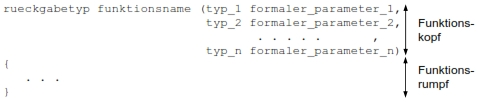
\includegraphics[width=1\textwidth]{pics/funktionen_aufbau.jpg}
		\end{minipage}
		%
		\begin{minipage}[c]{9 cm}
			\begin{compactitem}
				\item Funktionskopf: legt die Aufrufschnittstelle (Signatur) der Funktion fest. Er besteht aus R�ckgabetyp, Funktionsname und Parameterliste.
				\item Funktionsrumpf: Lokale Vereinbarungen und Anweisungen innerhalb eines Blocks
			\end{compactitem}	
		\end{minipage}	
			
	\subsection{Eingaben/Ausgaben einer Funktion \verweisboth{9.3}{7.3}}
		\begin{minipage}[t]{8.5 cm}
			\subsubsection{Eingabedaten}
				Es sind folgende M�glichkeiten vorhanden um Daten an Funktionen zu �bergeben:
				\begin{compactitem}
					\item Mithilfe von Werten, welche an die Parameterliste �bergeben werden
					\item Mithilfe von globalen Variablen
				\end{compactitem}
		\end{minipage}
		\hspace*{0.5cm}
		\begin{minipage}[t]{8.5 cm}
			\subsubsection{Ausgabedaten}
				Es sind folgende M�glichkeiten vorhanden um Daten zur�ckzugeben:
				\begin{compactitem}
					\item Mithilfe des R�ckgabewertes einer Funktion ($return$)
					\item Mithilfe von �nderungen an Variablen, deren Adresse �ber die Parameterliste an die Funktion �bergeben wurde
					\item Mithilfe von �nderungen an globalen Variablen
				\end{compactitem}	
		\end{minipage}	
		
		\subsubsection{Beispiele}
			\begin{minipage}[t]{8.5 cm}
				\textbf{Parameterlos und ohne R�ckgabewert:}
				\lstinputlisting[language=C,tabsize=2]{code/funktionen_parameter_1.c}
				
				\textbf{Parameter und ohne R�ckgabewert:}
				\lstinputlisting[language=C,tabsize=2]{code/funktionen_parameter_2.c}
			\end{minipage}
			\hspace*{0.5cm}
			\begin{minipage}[t]{8.5 cm}
				\textbf{Parameter und R�ckgabewert:}
				\lstinputlisting[language=C,tabsize=2]{code/funktionen_parameter_3.c}
			\end{minipage}

	\subsection{Deklaration von Funktionen \verweisboth{9.4}{7.2}}
		Es ist festgelegt, dass die Konsistenz zwischen Funktionskopf und Funktionsaufrufen vom Compiler �berpr�ft werden soll. Dazu muss beim Aufruf der Funktion die Schnittstelle der Funktion, d.h. der Funktionskopf, bereits bekannt sein. Steht aber die Definition einer Funktion im Programmcode erst nach ihrem Aufruf, so muss eine Vorw�rtsdeklaration der Funktion erfolgen, indem vor dem Aufruf die Schnittstelle der Funktion mit dem Funktionsprototypen deklariert wird. \\
		Desweitern ist zu beachten, dass Parameternamen im Funktionsprototyp und in der Funktionsdefinition nicht �bereinstimmen m�ssen. Es ist jedoch zu empfehlen.
		
		\begin{minipage}[t]{9.5 cm}
			\subsubsection{Beispiel}
				\lstinputlisting[language=C,tabsize=2]{code/funktionen_prototyp.c}	
		\end{minipage}
		\hspace*{0.5cm}
		\begin{minipage}[t]{7.5 cm}	
			\subsubsection{Was passiert wenn der Prototyp vergessen geht?}
				\begin{compactitem}
					\item Fehlt der Prototyp ganz, so wird die Funktion implizit (automatisch vom System) deklariert. Ihr R�ckgabetyp wird als $int$ angenommen, die Parameter werden nicht �berpr�ft.
					\item Wenn die Funktion sp�ter definiert wird und nicht $int$ als R�ckgabetyp hat, bringt der Compiler eine Fehlermeldung.
				\end{compactitem}
		\end{minipage}
		
		\subsubsection{Funktionsprototypen in der Praxis \verweisc{9.4}}
			\begin{compactitem}
				\item Funktionsprototypen, welche die Schnittstelle der Unit beschreiben, kommen in das entsprechenden Headerfile.
				\item Jedes C-File, welches diese Schnittstelle nutzt, inkludiert dieses Headerfile und somit die Funktionsprototypen.
				\item Funktionsprototypen von internen Funktionen der Unit werden zuoberst im C-File aufgelistet und kommen nicht ins Headerfile.
			\end{compactitem}
			
	\subsection{$inline$-Funktionen vs. $C$-Makros \verweiscpp{7.5}}
		\begin{minipage}[t]{7 cm}
			\subsubsection{$C$-Makros}
				\begin{compactitem}
					\item $C$-Makros werden definiert mit $\#define$.
					\item $C$-Makros bewirken eine reine Textersetzung ohne jegliche Typenpr�fung.
					\item Bei Nebeneffekten (welche zwar vermieden werden sollten) verhalten sich Makros nicht wie beabsichtigt.
					\item $C$-Makros l�sen zwar das Problem mit dem Overhead, sind aber sehr unsicher.				
				\end{compactitem}
				\lstinputlisting[language=C,tabsize=2]{code/c_makro.c}
			\end{minipage}
			\hspace*{0.5cm}
			\begin{minipage}[t]{10 cm}	
				\subsubsection{$inline$-Funktionen}
					\begin{compactitem}
						\item L�sen das Overhead-Problem.
						\item Der Code wird direkt eingef�gt, kein Funktionsaufruf findet statt.
						\item Eine Typenpr�fung wird durchgef�hrt.
						\item Einsetzen wenn der Codeumfang der Funktion sehr klein ist und die Funktion h�ufig aufgerufen wird (z.B. in Schleifen).
						\item Rekursive Funktionen und Funktionen, auf die mit einem Funktionspointer gezeigt wird, werden nicht $inlined$.
					\end{compactitem}
					\lstinputlisting[language=C++,tabsize=2]{code/inline.cpp}
			\end{minipage}	
		
	\subsection{Vorbelegte Parameter \verweiscpp{7.6}}
		\begin{compactitem}
		\end{compactitem}